\chapter{Implementation}
% How the implementation was done and tested, with particular focus on important / novel algorithms and/or data structures, unusual implementation decisions, novel user interface features, etc.
% General Introduction: Language used. How it linked to the task. How the task progressed over time. Any changes over time.
% Specific Sections: Goal of each part. Purpose or context within larger whole. How each part works step by step. (STAR?)
\section{Cells}
\subsection{Cell Class}\label{sec:cellClass}
The cell class contains integer coordinates, a set of possible tile options and a tile prefab game object. These variables allow the cell to be used in a grid for level generation. The set of tile options is initialised with the entire fully-explicit tile set. As WFC is run on a grid including the cell, tiles that become invalid options are removed. Once the cell has been collapsed, the assigned tile is instantiated. Additionally a reference to the instantiated tile is preserved in the tile prefab field.

% Diagram of a Cell, showing its list of possible tile choices.
\begin{figure}[H]
    \centering
    \subfigure[Cell]{
        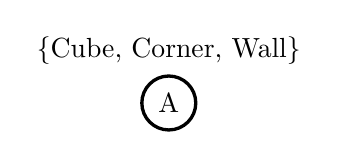
\begin{tikzpicture}[circlenode/.style={circle, draw=black, very thick, minimum size=5mm}]
            %Nodes
            \node[circlenode, label={[align=center]\{Cube, Corner, Wall\}}]      (00)                                            {A};

            %Lines
        \end{tikzpicture}
        \label{fig:tileOptions1}
    }

    \vspace{\baselineskip} % add some vertical space between the rows

    \subfigure[Cube Tile]{
        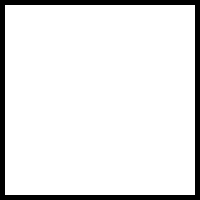
\includegraphics[width=0.2375\textwidth, height=0.1\textheight, keepaspectratio]{Images/CubeTile.png}
        \label{fig:tileOptions2}
    }
    \hfill
    \subfigure[Corner Tile]{
        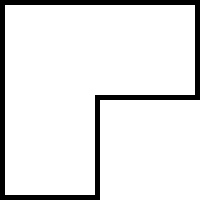
\includegraphics[width=0.2375\textwidth, height=0.1\textheight, keepaspectratio]{Images/CornerTile.png}
        \label{fig:tileOptions3}
    }
    \hfill
    \subfigure[Wall Tile]{
        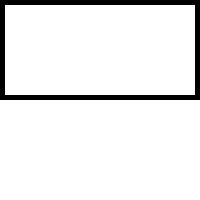
\includegraphics[width=0.2375\textwidth, height=0.1\textheight, keepaspectratio]{Images/WallTile.png}
        \label{fig:tileOptions4}
    }
    \caption{A cell with cube, corner and wall tiles as options}
    \label{fig:tileOptions}
\end{figure}

One additional property to note is that the cell class does not inherit from Unity's MonoBehaviour class. This means that it can use constructors that pass basic information needed to initialise each cell. Initialisation data includes the coordinates of the cell within the current layer, the cell's global grid coordinates and the current chunk using the cell. This data is needed for constraint calculations while solving and is updated each time a new layer is spawned.

Objects that do inherit from MonoBehaviour cannot use constructors safely and must instead use Unity's Start or Awake functions. However, the Start and Awake functions cannot easily be passed initialisation data. The cost of not inheriting from MonoBehaviour is that any such instances cannot be attached to any objects spawned in the world.

\subsection{CellArc Class}
The cell arc class is used to represent arcs in the grid. Each arc contains references to two cells. The constructor is used to ensure that the arc is valid. This is done by comparing the x and y coordinates of the cells when creating the arc. An exception is thrown when the cells are not adjacent. Cells being adjacent is specific to the context of WFC. In Sudoku, for example, a pair of constrained cells need not be directly adjacent.

% Show two cells and their arc.

\subsection{CellReference Class}\label{sec:cellReferenceClass}
The cell reference class contains a reference to a cell. As mentioned in Section \ref{sec:cellClass}, the cell class does not inherit from MonoBehaviour and as such cannot be attached to any objects in the world. By instead inheriting from MonoBehaviour, a cell reference instance can be attached to a tile. Having this cell reference attached to a tile allows the cell's data to be used in generation of later layers.

% Screenshot of CellReference on generated tile in Unity?

\section{Tiles}
\subsection{Rotation / Cardinality}
Each spawned tile has a cardinality of either 0, 1, 2 or 3. These cardinalities correspond to rotations of 0, 90, 180 and 270 degrees respectively. As example, all cardinalities for the corner tile are shown in Figure \ref{fig:cornerCardinalities}.

% Show corner tile with cardinalities 0, 1, 2 and 3.\begin{figure}[H]
\begin{figure}[H]
    \centering
    \subfigure[Cardinality 0 (0 Degrees)]{
        \rotatebox[origin=c]{-0}{
            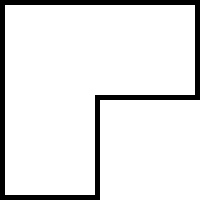
\includegraphics[width=0.2375\textwidth, height=0.1\textheight, keepaspectratio]{Images/CornerTile.png}
        }
        \label{fig:cornerCardinalities0}
    }
    \hfill
    \subfigure[Cardinality 1 (90 Degrees)]{
        \rotatebox[origin=c]{-90}{
            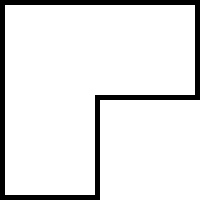
\includegraphics[width=0.2375\textwidth, height=0.1\textheight, keepaspectratio]{Images/CornerTile.png}
        }
        \label{fig:cornerCardinalities1}
    }
    \hfill
    \subfigure[Cardinality 2 (180 Degrees)]{
        \rotatebox[origin=c]{-180}{
            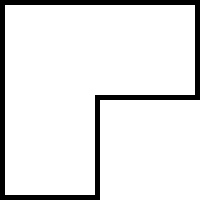
\includegraphics[width=0.2375\textwidth, height=0.1\textheight, keepaspectratio]{Images/CornerTile.png}
        }
        \label{fig:cornerCardinalities2}
    }
    \hfill
    \subfigure[Cardinality 3 (270 Degrees)]{
        \rotatebox[origin=c]{-270}{
            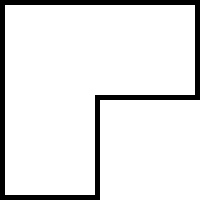
\includegraphics[width=0.2375\textwidth, height=0.1\textheight, keepaspectratio]{Images/CornerTile.png}
        }
        \label{fig:cornerCardinalities3}
    }
    \caption{The corner tile with all possible rotations (counted clockwise)}
    \label{fig:cornerCardinalities}
\end{figure}

Cardinality information is used to determine which combination of two tiles and their rotations fit together. For example, a single wall tile constituting part of a longer wall will require any adjacent wall tiles to be of the same cardinality as in Figure \ref{fig:wallExample1}. When specifying the neighbours of a tile, the level designer must also set the cardinality of each neighbour.

% Also show wall tiles fitting together. 0,0,0 walls fit and 3,0,1 walls don't.
\begin{figure}[H]
    \centering
    \subfigure[Valid wall placement (Cardinalities 0,0,0,0)]{
        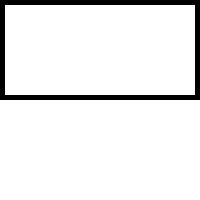
\includegraphics[width=0.2375\textwidth, height=0.1\textheight, keepaspectratio]{Images/WallTile.png}
        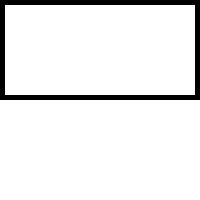
\includegraphics[width=0.2375\textwidth, height=0.1\textheight, keepaspectratio]{Images/WallTile.png}
        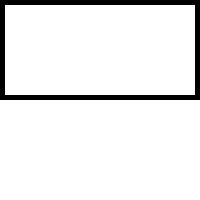
\includegraphics[width=0.2375\textwidth, height=0.1\textheight, keepaspectratio]{Images/WallTile.png}
        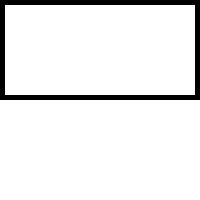
\includegraphics[width=0.2375\textwidth, height=0.1\textheight, keepaspectratio]{Images/WallTile.png}
        \label{fig:wallExample1}
    }

    \vspace{\baselineskip} % add some vertical space between the rows

    \subfigure[Invalid wall placement (Cardinalities 3,0,2,1)]{
        \rotatebox[origin=c]{-270}{
            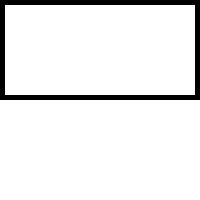
\includegraphics[width=0.2375\textwidth, height=0.1\textheight, keepaspectratio]{Images/WallTile.png}
        }
        \rotatebox[origin=c]{-0}{
            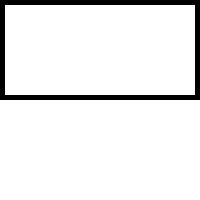
\includegraphics[width=0.2375\textwidth, height=0.1\textheight, keepaspectratio]{Images/WallTile.png}
        }
        \rotatebox[origin=c]{-180}{
            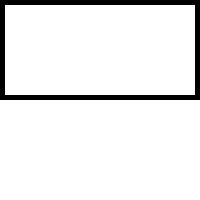
\includegraphics[width=0.2375\textwidth, height=0.1\textheight, keepaspectratio]{Images/WallTile.png}
        }
        \rotatebox[origin=c]{-90}{
            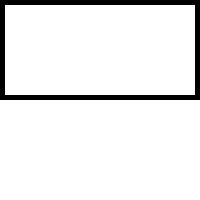
\includegraphics[width=0.2375\textwidth, height=0.1\textheight, keepaspectratio]{Images/WallTile.png}
        }
        \label{fig:wallExample2}
    }
    \caption{Comparison of valid wall placement to invalid wall placement if adjacent walls must have matching cardinality}
    \label{fig:wallExample}
\end{figure}

\subsection{Tile Symmetry}\label{sec:tileSymmetry}
To reduce the amount of adjacency data to be specified by the level designer, as well as the chance for human error, the level generator includes the functionality to convert a semi-explicit tile set into a fully-explicit tile set. This fully-explicit tile set is created at the start of generation in several steps.

First, it is checked whether the empty tile was specified and is included in the semi-explicit tile set. After confirming this, the main conversion stage begins.

Second, a non-symmetric copy is created for each tile. Non-symmetric tiles may have different neighbours on each side. Any symmetric tile can be represented as a non-symmetric tile. For example, a tile with equal symmetry on all sides can be converted by copying the single list of neighbours onto all sides and incrementing the cardinality per side as required. Specifically, cardinalities on side 1 are incremented by 1, those on side 2 by 2 and those on side 3 by 3. This fully symmetric tile is called a cube tile in the code.

% Image of cube with wall neighbour being turned into non-symmetric tile.
\begin{figure}[H]
    \subfigure[A symmetric cube tile with only a wall neighbour of cardinality 2 on the back side specified]{
        \begin{minipage}[b]{0.45\linewidth}
            \centering
            \rotatebox[origin=c]{-180}{
                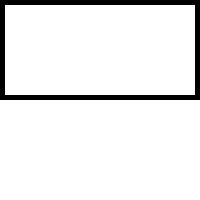
\includegraphics[width=0.2375\textwidth, height=0.1\textheight, keepaspectratio]{Images/WallTile.png}
            }

            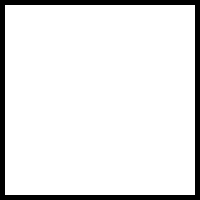
\includegraphics[width=0.2375\textwidth, height=0.1\textheight, keepaspectratio]{Images/CubeTile.png}

            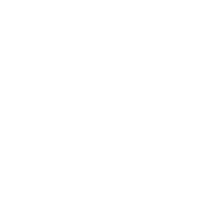
\includegraphics[width=0.2375\textwidth, height=0.1\textheight, keepaspectratio]{Images/EmptyTile.png}
        \end{minipage}
        \label{fig:cubeSymmetryConversion1}
    }
    \hfill
    \subfigure[A non-symmetric cube tile variant with a wall neighbour specified on each side. Clockwise from the back, cardinalities of the walls are 2, 3, 0 and 1.]{
        \begin{minipage}[b]{0.45\linewidth}
            \centering
            \rotatebox[origin=c]{-180}{
                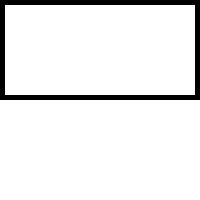
\includegraphics[width=0.2375\textwidth, height=0.1\textheight, keepaspectratio]{Images/WallTile.png}
            }

            \rotatebox[origin=c]{-90}{
                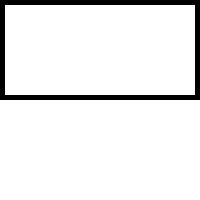
\includegraphics[width=0.2375\textwidth, height=0.1\textheight, keepaspectratio]{Images/WallTile.png}
            }
            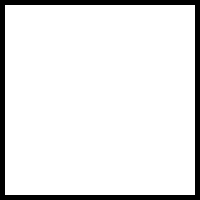
\includegraphics[width=0.2375\textwidth, height=0.1\textheight, keepaspectratio]{Images/CubeTile.png}
            \rotatebox[origin=c]{-270}{
                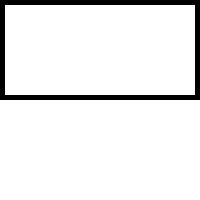
\includegraphics[width=0.2375\textwidth, height=0.1\textheight, keepaspectratio]{Images/WallTile.png}
            }

            \rotatebox[origin=c]{-0}{
                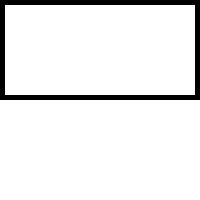
\includegraphics[width=0.2375\textwidth, height=0.1\textheight, keepaspectratio]{Images/WallTile.png}
            }
        \end{minipage}
        \label{fig:cubeSymmetryConversion2}
    }
    \caption{A symmetric cube tile converted to a non-symmetric tile. For simplicity, the cube is only shown with a wall as its possible neighbour.}
    \label{fig:cubeSymmetryConversion}
\end{figure}

Third, an array for each possible tile rotation is created (cardinalities 0, 1, 2 and 3). This array is attached to the original tile to set explicit neighbours later. The instantiated tile is used as the base rotation (cardinality 0) and referenced in the array. For cube tiles, the base rotation tile can be referenced for each rotation instead of having to create additional copies. The filled in array for cube tiles is shown in Figure \ref{fig:cubeRotationsArray}.

% Show the rotations array for the cube tile and how it is just the same in each slot.
\begin{figure}[H]
    \subfigure[Cube Tile Explicit Variant 0]{
        \begin{minipage}[b]{0.22\linewidth}
            \centering
            \rotatebox[origin=c]{-180}{
                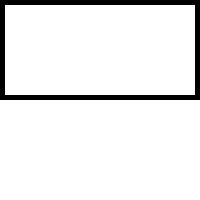
\includegraphics[width=0.2375\textwidth, height=0.1\textheight, keepaspectratio]{Images/WallTile.png}
            }

            \rotatebox[origin=c]{-90}{
                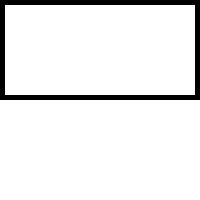
\includegraphics[width=0.2375\textwidth, height=0.1\textheight, keepaspectratio]{Images/WallTile.png}
            }
            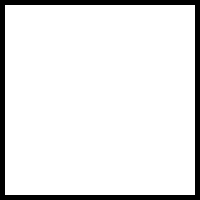
\includegraphics[width=0.2375\textwidth, height=0.1\textheight, keepaspectratio]{Images/CubeTile.png}
            \rotatebox[origin=c]{-270}{
                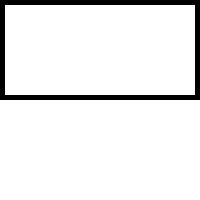
\includegraphics[width=0.2375\textwidth, height=0.1\textheight, keepaspectratio]{Images/WallTile.png}
            }

            \rotatebox[origin=c]{-0}{
                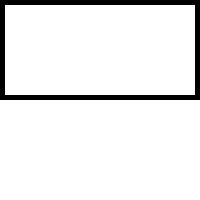
\includegraphics[width=0.2375\textwidth, height=0.1\textheight, keepaspectratio]{Images/WallTile.png}
            }
        \end{minipage}
        \label{fig:cubeRotationsArray0}
    }
    \hfill
    \subfigure[Cube Tile Explicit Variant 1]{
        \begin{minipage}[b]{0.22\linewidth}
            \centering
            \rotatebox[origin=c]{-180}{
                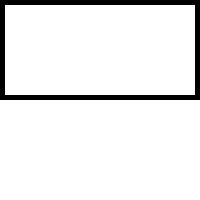
\includegraphics[width=0.2375\textwidth, height=0.1\textheight, keepaspectratio]{Images/WallTile.png}
            }

            \rotatebox[origin=c]{-90}{
                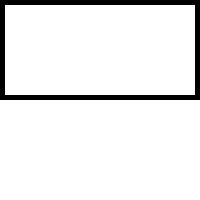
\includegraphics[width=0.2375\textwidth, height=0.1\textheight, keepaspectratio]{Images/WallTile.png}
            }
            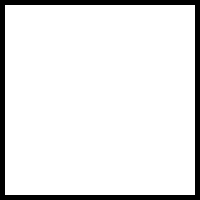
\includegraphics[width=0.2375\textwidth, height=0.1\textheight, keepaspectratio]{Images/CubeTile.png}
            \rotatebox[origin=c]{-270}{
                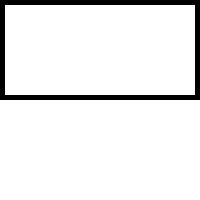
\includegraphics[width=0.2375\textwidth, height=0.1\textheight, keepaspectratio]{Images/WallTile.png}
            }

            \rotatebox[origin=c]{-0}{
                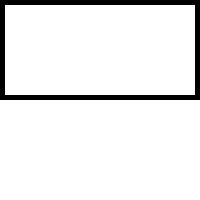
\includegraphics[width=0.2375\textwidth, height=0.1\textheight, keepaspectratio]{Images/WallTile.png}
            }
        \end{minipage}
        \label{fig:cubeRotationsArray1}
    }
    \hfill
    \subfigure[Cube Tile Explicit Variant 2]{
        \begin{minipage}[b]{0.22\linewidth}
            \centering
            \rotatebox[origin=c]{-180}{
                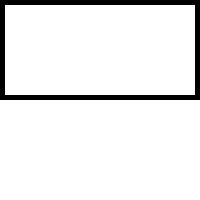
\includegraphics[width=0.2375\textwidth, height=0.1\textheight, keepaspectratio]{Images/WallTile.png}
            }

            \rotatebox[origin=c]{-90}{
                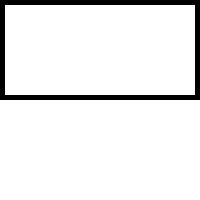
\includegraphics[width=0.2375\textwidth, height=0.1\textheight, keepaspectratio]{Images/WallTile.png}
            }
            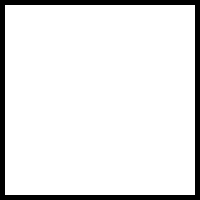
\includegraphics[width=0.2375\textwidth, height=0.1\textheight, keepaspectratio]{Images/CubeTile.png}
            \rotatebox[origin=c]{-270}{
                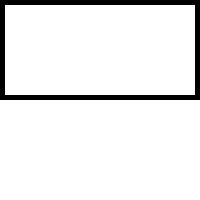
\includegraphics[width=0.2375\textwidth, height=0.1\textheight, keepaspectratio]{Images/WallTile.png}
            }

            \rotatebox[origin=c]{-0}{
                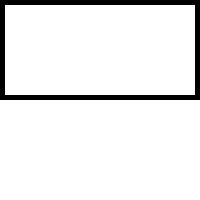
\includegraphics[width=0.2375\textwidth, height=0.1\textheight, keepaspectratio]{Images/WallTile.png}
            }
        \end{minipage}
        \label{fig:cubeRotationsArray2}
    }
    \hfill
    \subfigure[Cube Tile Explicit Variant 3]{
        \begin{minipage}[b]{0.22\linewidth}
            \centering
            \rotatebox[origin=c]{-180}{
                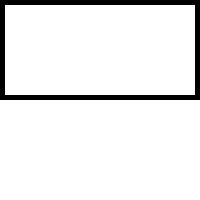
\includegraphics[width=0.2375\textwidth, height=0.1\textheight, keepaspectratio]{Images/WallTile.png}
            }

            \rotatebox[origin=c]{-90}{
                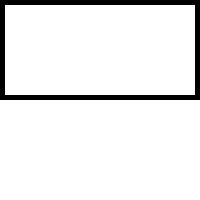
\includegraphics[width=0.2375\textwidth, height=0.1\textheight, keepaspectratio]{Images/WallTile.png}
            }
            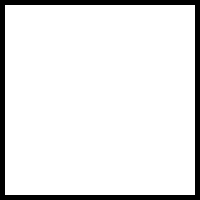
\includegraphics[width=0.2375\textwidth, height=0.1\textheight, keepaspectratio]{Images/CubeTile.png}
            \rotatebox[origin=c]{-270}{
                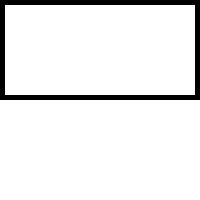
\includegraphics[width=0.2375\textwidth, height=0.1\textheight, keepaspectratio]{Images/WallTile.png}
            }

            \rotatebox[origin=c]{-0}{
                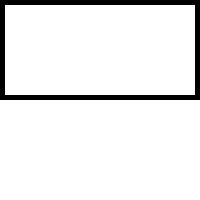
\includegraphics[width=0.2375\textwidth, height=0.1\textheight, keepaspectratio]{Images/WallTile.png}
            }
        \end{minipage}
        \label{fig:cubeRotationsArray3}
    }
    \caption{The array of explicit variants for the cube tile with neighbours shown. Due to the tile's symmetry, no extra work is needed to calculate variants for cardinalities 1, 2 and 3.}
    \label{fig:cubeRotationsArray}
\end{figure}

For non-cube tiles, variants for the remaining cardinalities (1, 2 and 3) must be created. Each new variant copies the previous one. This allows a loop to be used that always performs 90 degree steps. First, the tile is rotated by 90 degrees. Then, neighbour data and rotation arrays are swapped. This sets back neighbours as left neighours, left neighbours as front neighbours and so on. Finally, the cardinality values of all neighbours are incremented by 1 to mark the 90 degree rotation. The filled in array for corner tiles is shown in Figure \ref{fig:cornerRotationsArray}.

% Show the rotations array for the corner tile. Show cardinality 0 corner rotated to cardinality 1 corner etc.
\begin{figure}[H]
    \subfigure[Corner Tile Explicit Variant 0]{
        \begin{minipage}[b]{0.22\linewidth}
            \centering
            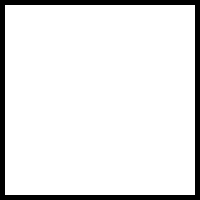
\includegraphics[width=0.2375\textwidth, height=0.1\textheight, keepaspectratio]{Images/CubeTile.png}

            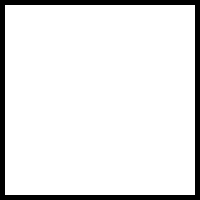
\includegraphics[width=0.2375\textwidth, height=0.1\textheight, keepaspectratio]{Images/CubeTile.png}
            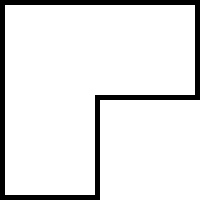
\includegraphics[width=0.2375\textwidth, height=0.1\textheight, keepaspectratio]{Images/CornerTile.png}
            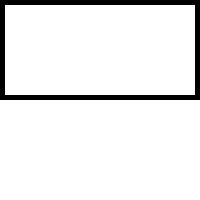
\includegraphics[width=0.2375\textwidth, height=0.1\textheight, keepaspectratio]{Images/WallTile.png}

            \rotatebox[origin=c]{-270}{
                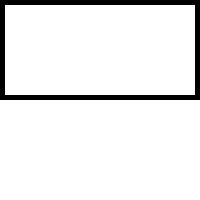
\includegraphics[width=0.2375\textwidth, height=0.1\textheight, keepaspectratio]{Images/WallTile.png}
            }
        \end{minipage}
        \label{fig:cornerRotationsArray0}
    }
    \hfill
    \subfigure[Corner Tile Explicit Variant 1]{
        \begin{minipage}[b]{0.22\linewidth}
            \centering
            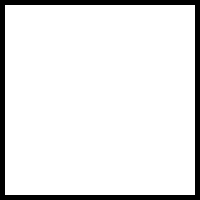
\includegraphics[width=0.2375\textwidth, height=0.1\textheight, keepaspectratio]{Images/CubeTile.png}

            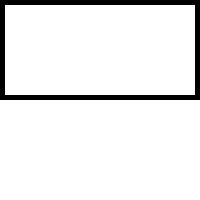
\includegraphics[width=0.2375\textwidth, height=0.1\textheight, keepaspectratio]{Images/WallTile.png}
            \rotatebox[origin=c]{-90}{
                \includegraphics[width=0.2375\textwidth, height=0.1\textheight, keepaspectratio]{Images/CornerTile.png}
            }
            \includegraphics[width=0.2375\textwidth, height=0.1\textheight, keepaspectratio]{Images/CubeTile.png}

            \rotatebox[origin=c]{-90}{
                \includegraphics[width=0.2375\textwidth, height=0.1\textheight, keepaspectratio]{Images/WallTile.png}
            }
        \end{minipage}
        \label{fig:cornerRotationsArray1}
    }
    \hfill
    \subfigure[Corner Tile Explicit Variant 2]{
        \begin{minipage}[b]{0.22\linewidth}
            \centering
            \rotatebox[origin=c]{-90}{
                \includegraphics[width=0.2375\textwidth, height=0.1\textheight, keepaspectratio]{Images/WallTile.png}
            }

            \rotatebox[origin=c]{-180}{
                \includegraphics[width=0.2375\textwidth, height=0.1\textheight, keepaspectratio]{Images/WallTile.png}
            }
            \rotatebox[origin=c]{-180}{
                \includegraphics[width=0.2375\textwidth, height=0.1\textheight, keepaspectratio]{Images/CornerTile.png}
            }
            \includegraphics[width=0.2375\textwidth, height=0.1\textheight, keepaspectratio]{Images/CubeTile.png}

            \includegraphics[width=0.2375\textwidth, height=0.1\textheight, keepaspectratio]{Images/CubeTile.png}
        \end{minipage}
        \label{fig:cornerRotationsArray2}
    }
    \hfill
    \subfigure[Corner Tile Explicit Variant 3]{
        \begin{minipage}[b]{0.22\linewidth}
            \centering
            \rotatebox[origin=c]{-270}{
                \includegraphics[width=0.2375\textwidth, height=0.1\textheight, keepaspectratio]{Images/WallTile.png}
            }

            \includegraphics[width=0.2375\textwidth, height=0.1\textheight, keepaspectratio]{Images/CubeTile.png}
            \rotatebox[origin=c]{-270}{
                \includegraphics[width=0.2375\textwidth, height=0.1\textheight, keepaspectratio]{Images/CornerTile.png}
            }
            \rotatebox[origin=c]{-180}{
                \includegraphics[width=0.2375\textwidth, height=0.1\textheight, keepaspectratio]{Images/WallTile.png}
            }

            \includegraphics[width=0.2375\textwidth, height=0.1\textheight, keepaspectratio]{Images/CubeTile.png}
        \end{minipage}
        \label{fig:cornerRotationsArray3}
    }
    \caption{The array of explicit variants for the corner tile with neighbours shown.}
    \label{fig:cornerRotationsArray}
\end{figure}

These explicit variants do not yet have tile rotation implicitly encoded in their neighbour data. The original tile neighbours in the tile array must be replaced with their explicit variants matching the rotations in the rotations array. To do this, the array assigned to each tile containing all the explicit variants is used once all explicit variants have been created. For each neighbour of the explicit tile, the reference to the non-explicit neighbour is replaced by the explicit neighbour with the correct orientation. As example, the explicit corner tile variants are shown with the original cube and wall neighbours in Figure \ref{fig:explicitNeighbourUpdate}. The references are changed to explicit cube and wall neighbours to match Figure \ref{fig:cornerRotationsArray}.

% Diagram of this process. Show the original tile and each variant in a line. Then show how the neighbours of one of these is replaced with the explicit variants.
\begin{figure}[H]
    \subfigure[Corner Tile Explicit Variant 0 Before Neighbour Update]{
        \begin{minipage}[b]{0.22\linewidth}
            \centering
            \includegraphics[width=0.2375\textwidth, height=0.1\textheight, keepaspectratio]{Images/CubeTile.png}

            \includegraphics[width=0.2375\textwidth, height=0.1\textheight, keepaspectratio]{Images/CubeTile.png}
            \includegraphics[width=0.2375\textwidth, height=0.1\textheight, keepaspectratio]{Images/CornerTile.png}
            \includegraphics[width=0.2375\textwidth, height=0.1\textheight, keepaspectratio]{Images/WallTile.png}

            \includegraphics[width=0.2375\textwidth, height=0.1\textheight, keepaspectratio]{Images/WallTile.png}
        \end{minipage}
        \label{fig:explicitNeighbourUpdate0}
    }
    \hfill
    \subfigure[Corner Tile Explicit Variant 1 Before Neighbour Update]{
        \begin{minipage}[b]{0.22\linewidth}
            \centering
            \includegraphics[width=0.2375\textwidth, height=0.1\textheight, keepaspectratio]{Images/CubeTile.png}

            \includegraphics[width=0.2375\textwidth, height=0.1\textheight, keepaspectratio]{Images/WallTile.png}
            \rotatebox[origin=c]{-90}{
                \includegraphics[width=0.2375\textwidth, height=0.1\textheight, keepaspectratio]{Images/CornerTile.png}
            }
            \includegraphics[width=0.2375\textwidth, height=0.1\textheight, keepaspectratio]{Images/CubeTile.png}

            \includegraphics[width=0.2375\textwidth, height=0.1\textheight, keepaspectratio]{Images/WallTile.png}
        \end{minipage}
        \label{fig:explicitNeighbourUpdate1}
    }
    \hfill
    \subfigure[Corner Tile Explicit Variant 2 Before Neighbour Update]{
        \begin{minipage}[b]{0.22\linewidth}
            \centering
            \includegraphics[width=0.2375\textwidth, height=0.1\textheight, keepaspectratio]{Images/WallTile.png}

            \includegraphics[width=0.2375\textwidth, height=0.1\textheight, keepaspectratio]{Images/WallTile.png}
            \rotatebox[origin=c]{-180}{
                \includegraphics[width=0.2375\textwidth, height=0.1\textheight, keepaspectratio]{Images/CornerTile.png}
            }
            \includegraphics[width=0.2375\textwidth, height=0.1\textheight, keepaspectratio]{Images/CubeTile.png}

            \includegraphics[width=0.2375\textwidth, height=0.1\textheight, keepaspectratio]{Images/CubeTile.png}
        \end{minipage}
        \label{fig:explicitNeighbourUpdate2}
    }
    \hfill
    \subfigure[Corner Tile Explicit Variant 3 Before Neighbour Update]{
        \begin{minipage}[b]{0.22\linewidth}
            \centering
            \includegraphics[width=0.2375\textwidth, height=0.1\textheight, keepaspectratio]{Images/WallTile.png}

            \includegraphics[width=0.2375\textwidth, height=0.1\textheight, keepaspectratio]{Images/CubeTile.png}
            \rotatebox[origin=c]{-270}{
                \includegraphics[width=0.2375\textwidth, height=0.1\textheight, keepaspectratio]{Images/CornerTile.png}
            }
            \includegraphics[width=0.2375\textwidth, height=0.1\textheight, keepaspectratio]{Images/WallTile.png}

            \includegraphics[width=0.2375\textwidth, height=0.1\textheight, keepaspectratio]{Images/CubeTile.png}
        \end{minipage}
        \label{fig:explicitNeighbourUpdate3}
    }
    \caption{The explicit corner tile variants before updating neighbours to their explicit forms}
    \label{fig:explicitNeighbourUpdate}
\end{figure}

% // Initialise the explicit tile set if it has not already been done.
% // Ensure that the empty tile is in the tile set.
% // Create a game object to hold the explicit tile set.
% // Create non-symmetric variants for each tile.
% // Create a non-symmetric copy of the original tile.
% // Add the copy to the explicit tile set and set it as the 0 rotation variant.
% // Set the explicit variant of the empty tile if applicable.
%%%IF // Create rotation variants for non-cube tiles.
% // Create a rotation variant with the previous rotation as the base.
% // Rotate the variant by 90 degrees and specify its rotation / cardinality in the name.
% // Add the variant to both the tile's variants array and the explicit tile set.
% // Switch the neighbour and rotation arrays to follow the 90 degree rotation.
% // Increase cardinality values of neighbours to account for the 90 degree rotation.
%%%ELSE // For cube tiles, simply set the explicit rotation variants to be the 0 rotation non-symmetric tile.
% // Replace the neighbours of each explicit tile without explicit rotational information with explicit variants accounting for the rotations.
% // Use 2D arrays of the neighbours and rotations to simplify the operation.
% // Go through each neighbour array and neighbour tile in it.
% // Get the rotation / cardinality value of the variant to use.
% // Set the neighbour to the explicit variant with the correct rotation.

\subsection{Collapsing Cells}\label{sec:collapsingCells}
To collapse a tile into a cell, the tile's model is instantiated. Then, the model is set to follow the level generation manager's transform (position, rotation and scale) and has its local position reset to the cell's world coordinates. Doing the placement in this way ensures that the model lines up with the world grid while maintaining the correct scale and rotation. Finally, a Unity box collider is added to the model, a second reference to the tile added to the cell and the model activated to render it in the world. The second reference ensures that the spawned tile can be recovered if the generation of a layer fails. Unity's `Physics.OverlapBox' function can be used to detect the box collider given the world coordinates of the cell. This box overlap can be used to obtain the cell reference during the generation of later layers.

% Diagram of the pipeline.
% Instantiate, place, add collider, reference and set active.

\section{Chunks}
Chunks are defined by their own chunk coordinates, which are converted from world coordinates using the chunk size as a divisor. From this, each of the chunk's four layers can be defined. Layer one is aligned with the chunk's world coordinates, while layer two is offset by half a chunk in the x direction. Layer three is similarly offset by half a chunk in the y direction, while layer four is offset both in the x and y directions. Each layer is given its own layer spawner instance, which runs WFC on the portion of the chunk defined by the layer.

% Chunk diagram with layer shown.

Each chunk has its own Random Number Generator (RNG), which is used by the layer spawners when making tile choices. The seed for the RNG is defined deterministically through the chunk's coordinates. The global level generation seed is added to allow generation of multiple levels while keeping determinism. This deterministic use of RNGs when spawning chunks is what allows the level generation manager to spawn chunks identically, even when unloading and loading a chunk again.

\section{Level Generation Manager}
\subsection{Prerequisites}
To start generation, the level designer must have defined a tile set for the generator to use. This must contain an empty tile and be convertible into an explicit tile set as detailed in Section \ref{sec:tileSymmetry}.

\subsection{Solver (Layer Spawners)}
The MAC3 solver code is held in the layer spawner class. This matches the idea of layers and chunks modifying the world in an infinite set of blocks. To allow accurate placement of tiles in the world, a starting cell coordinate must be passed when initialising the layer spawner. Furthermore, a reference to the layer's parent chunk is kept in order to utilise its random number generator.

\subsection{Grid Initialisation}
First, a grid of cells is initialised. Additionally, a list of cells left to assign is initialised to simplify cell choices when solving. Padding on the layer size is used to include any previously collapsed cells. Added cells that have not been collapsed are treated as empty tiles. This padding means that non-padded cells take into account full adjacency information. If the layer were not padded, then border cells would not have arc consistency with cells outside of the layer as these arcs would not be checked by the solver. The non-padding cells in the centre of the grid are refreshed by restoring each cell's tile options set to include all possible tiles. This allows each each layer to re-generate its cells. In effect, this connects singular, overlapping layers into an infinite, continuous grid.% WHY Are non-collapsed cells treated as empty tiles? DOES THIS HELP STITCHING? EXPERIMENT AGAIN AND WRITE DOWN REASONING.

\subsection{Dealing with an Infinite Grid}
Were every cell stored in a global grid, then it would be trivially easy to get previously collapsed cells. This is unfeasible due to the requirement of letting the player navigate an infinite world. As such, once cells are collapsed, the grid used by the solver is discarded. Instead, the cell reference class described in Section \ref{sec:cellReferenceClass} is used to preserve a reference to the cell. Each tile has its own collider that can be used to obtain the cell reference as described in Section \ref{sec:collapsingCells}.% DISCUSS ALTERNATIVE IN EVALUATION. MAYBE A "SEMI-GLOBAL" GRID THAT CONTAINS ALL THE CURRENTLY COLLAPSED CELLS AND SHIFTS AS THE PLAYER MOVES.

\subsection{Setting up MAC3}
With the layer's grid fully initialised, the main stage of the solver can now begin. First, a stack of state changes is initialised. This tracks changes to cells after each assignment by pushing a new state change to the stack. To make the grid globally arc consistent, the arc of each cell in the grid is generated. Subsequently, AC3 is run with this starting queue of cell arcs.

\subsection{MAC3 Recursion}
After this, the first iteration of a recursive implementation of the MAC3 algorithm is called. Pseudocode of this is given below. How each step works and its purpose is explained in more detail in subsections following the pseudocode.

\begin{enumerate}
    \item If all cells have been assigned, return.
    \item Choose a cell and tile to assign as in Section \ref{sec:variableAndValueChoice}.
    \item Enter a new state and assign the tile to the cell, pruning other tiles from its tile options set.
    \item If the cell's tile options set changed, run AC3.
    \item Recurse if AC3 was not run or there was no domain wipeout during AC3.
    \item If all cells have been assigned, return.
    \item We are now in the case that a domain wipeout must have occurred. Revert the state.
    \item If the cell we tried to assign still has other options left, remove / `unassign' the tile we tried from the options, run AC3 and recurse again.
    \item If all cells have been assigned, return.
    \item We are now in the case that all possible tile values for a cell led to a wipeout. This means that an earlier choice must be to blame. Restore the tile we tried both to assign and unassign and return.
\end{enumerate}

\subsubsection{Managing State Changes}
To track state changes, each layer spawner holds a stack of state changes. After each time a new cell is chosen to be assigned, a new state is entered. A state change class is used that holds the cell being assigned and any domain changes occurring across the grid. Domain changes can happen to any cell and can consist of multiple tile changes, so a dictionary of cells to hash sets of tiles is used. To track a new state change, a new entry and hash set are added to the dictionary if required. After this, the hash set can be obtained from the dictionary through use of the cell and any tile changes added.

% Image of domain changes structure.

To revert a state, the domain changes dictionary is iterated through, with each cell having any removed tiles restored to its domain. Furthermore, the cell that was assigned in the state change is re-added to the list of cells left to assign.

\subsubsection{Assigning and Unassigning a Tile to a Cell}
Assigning a tile to a cell involves pruning all tiles except the one being assigned. These tiles are removed from the tile options set. Furthermore, each domain change is recorded in the current state changes. Finally, the assigned cell is removed from the list of cells left to assign. After this, AC3 can be run to maintain arc consistency.

% Image of assignment.

Unassigning a tile to a cell first requires the state to be reverted. After this, the opposite choice is taken. This is done by pruning only the tile choice that was previously assigned. This demonstrates the 2-way branching nature of the implementation. Rather than exploring all possible tile values in one level of search, each tile value is either assigned or unassigned.

\subsubsection{Visualising Recursion}
The recursive MAC3 method can be visualised as consisting of three parts as in Figure \ref{fig:mac3Recursion}.

\begin{figure}[H]
    \begin{framed}
        \begin{enumerate}
            \item Making a new assignment.
            \item Making the opposite assignment (``unassignment'') after the first one failed.
            \item Both assignments having failed.
        \end{enumerate}
    \end{framed}
    \caption{The three parts of the recursive MAC3 method}
    \label{fig:mac3Recursion}
\end{figure}

The finishing state of the grid is checked both before making the new assignment and after each of the assignments. This ensures that the recursion is finished immediately after consistency has been enforced from an assignment and each cell only has one value left.